
\section{Navigation}

\subsection{1st Person Navigation Mode}

\TODO{ADD 1ST PERSON SHOT}
This widget has four moving directions and four rotations.
It allows to move forward/backward,
go up/down,
turn left/right and
pitch up/down.

Crossing a gate once starts the movement.
Crossing it again stops it.
If a gate is crossed while another one is active,
the first one stops -- this behavior was enforced
by user test inspection.
Having several moving/rotation
actions applied at the same this is confusing.
Clarity was favored over efficiency.

\subsection{Compass Navigation Mode}

\TODO{ADD COMPASS SHOT}

This is a direct application of the concept defined
in section \ref{sec:bev} Bird's Eye View Mode, on page \pageref{sec:bev}.

The outer ring of the widget allows the user to see and change
the current orientation in terms of cardial points positioning.

The inner circle allows inspection of the top-down view, with the user
being in the center. Applying strokes inside this area drags the map,
changing user's position in the ground plane.

\subsection{Examine Navigation Mode}

\TODO{ADD EXAMINE SHOT}

\TODO{ADD VIRTUAL SPHERE ILLUSTRATION}

This widget features a wire frame sphere at the center, two zooming gates
and two additional gates whole purpose is described below.
It is a direct application of the concept defined
in section \ref{sec:examine} Examine Navigation Mode, on page \pageref{sec:examine}.

The sphere occupying the center of the widget simulates the virtual sphere centered
on the subject of interest with radius $ dist $.

The user is at distance $ dist $ from the subject of interest.
This distance can be increased or decreased by activating the zoom gates.
Movements in the $ XX $ direction are translated into rotations around $ \theta $, while
movements in the $ YY $ direction translate into rotations around $ \phi $.

Two additional gates allow changing the subject of interest.
They work by crossing and ending the stroke at the target.
The first one, \emph{point of interest center}, allows one to examine the center of the object.
The remaining one, \emph{point of interest spot}, changes the examined position to be the surface
position where the stroke ``touches''.
The former is useful for inspection of the overall object while the latter is of great
use in editing or inspecting surface details.

\subsection{Fly Navigation Mode}

%intro DONE

\begin{figure}[!ht]
		\centering
		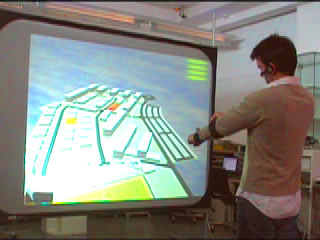
\includegraphics[width=6cm]{gfx/don.png}
		\caption{user navigating with the multimodal navigation mode}
		\label{fig:don}
\end{figure}

Navigation in a 3D scene takes place normally using a desktop computer
with the mouse and keyboard as input devices and the monitor as output device.
In the multimedia lab there was a motion tracking system available.
It was put to use in conjunction with a wireless microphone to allow for an
alternative mode of navigation. A set of reflective markers is attached to
the user's arms and the wireless microphone attached to his/her ear.
The microphone allows for enabling and disabling the multimodal navigation mode
by issuing respectively the commands \textbf{begin flying} / \textbf{stop flying}.

\subsubsection{Physical Configuration}

Motion tracking took place using reflective markers attached to the user's arms (figure \ref{fig:markers-cams} left).
A set of 4 cameras with infrared lights were installed in the lab, which each
captured image being processed by a computer identifying the visible markers in
image-space, making the computation of the spacial position of each marker by
merging the data from the 4 captured views and labeling each tracked marker
from the initial extended arm pose (figure \ref{fig:markers-cams} right).

The Microsoft Speech API 5.1, American English version was used to recognize the
voice commands. Capturing of the commands was done by attaching a wireless microphone
to the user's ear.

%ap�s a compara��o do reconhecimento do mesmo face a um microfone fixo e um Bluetooth.

%O reconhecedor mostrou-se algo limitado, tendo sido necess�rio adaptar a gram�tica a palavras n�o amb�guas entre si ou
%que gerassem falsos positivos.
%
%%Preliminarmente realizou-se um teste para escolher o melhor hardware para reconhecimento de voz, entre um microfone Wireless, %um fixo a captar toda a sala e um auricular Bluetooth. Os comandos dispon�veis na aplica��o foram ditados repetidas vezes por 3 %utilizadores, em ordem aleat�ria e com os 3 dispositivos.
%
%%Conclui-se que o microfone Wireless era a melhor op��o com uma taxa de reconhecimento m�dia de 99\%, mas para dist�ncias curtas %(\(<\)3m) o auricular Bluetooth teve resultados semelhantes, com 98\%. O microfone fixo captou muito ru�do e produziu resultados %muito insatisfat�rios de menos de 50\%.

%O reconhecedor mostrou-se algo limitado, tendo sido necess�rio adaptar a gram�tica a palavras n�o amb�guas entre si ou
%que gerassem falsos positivos.

\begin{figure}[!ht]
		\centering
		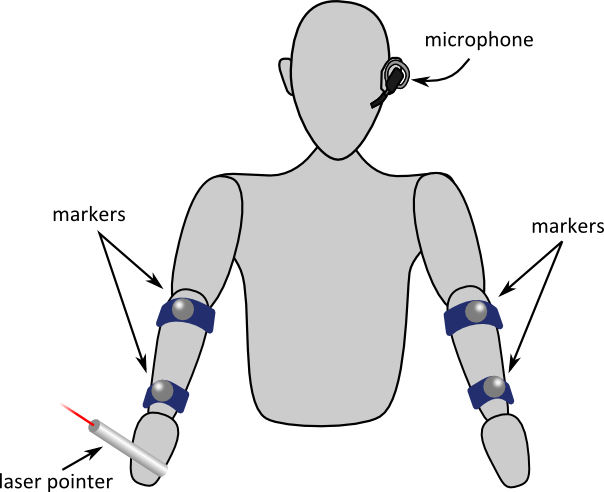
\includegraphics[width=7cm]{gfx/markers2.png}
		\qquad
		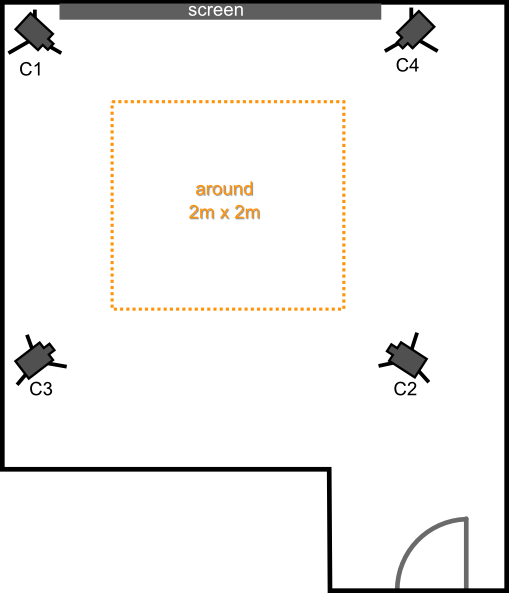
\includegraphics[width=5cm]{gfx/4cam-setup.png}
		\caption{markers and camera setup}
		\label{fig:markers-cams}
\end{figure}
%
%
%\begin{figure}[!ht]
%		\centering
%		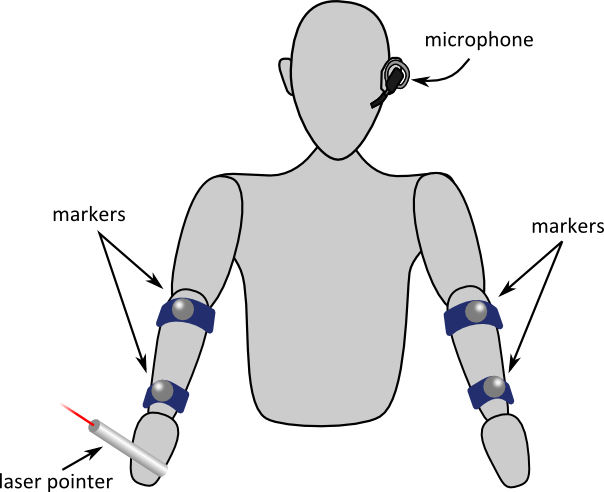
\includegraphics[width=6cm]{gfx/markers2.png}
%		\caption{markers and microphone for tracked user}
%		\label{fig:markers}
%\end{figure}
%
%\begin{figure}[!ht]
%		\centering
%		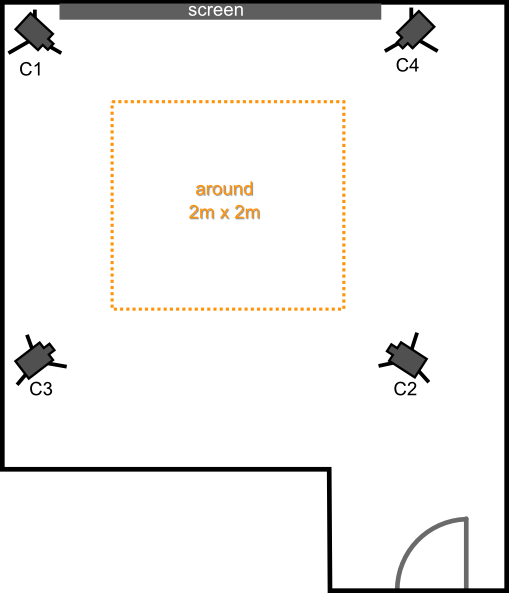
\includegraphics[width=6cm]{gfx/4cam-setup.png}
%		\caption{four cameras setup for motion tracking}
%		\label{fig:cam-setup}
%\end{figure}


\subsubsection{Interaction}

The multimodal navigation mode requires the user to have his / her arms extended towards the screen.

Controlling the flight speed works by the measurement of the distance between hands:
the closer they are from each other, the faster the flight speed is.
If the arms get close to a ninety degrees angle between them the flight halts (figure \ref{fig:fly-speed}).

Changing the flight orientation relatively to the ground plane is achieved by setting the arms
angle with the ground at opposing directions, with a bigger difference between angles generating
a faster rotation movement. If the user wants to turn right, for instance, he / she has to
raise the left arm and lower the right one (figure \ref{fig:fly-rot-up}, left).

To change flight altitude, both arms must be oriented in the same direction relatively to the ground plane,
either both raised or both lowered.
Again, the higher the angle is from the original arms extended forward pose,
the bigger the flight altitude shift occurs (figure \ref{fig:fly-rot-up}, right).

\begin{figure}[!ht]
		\centering
		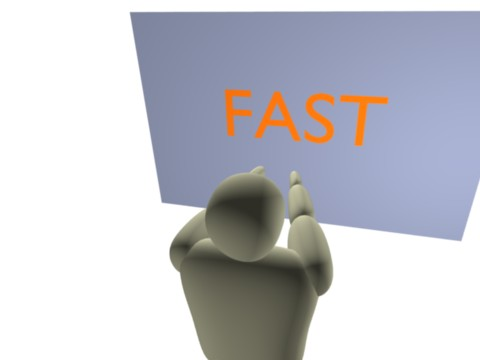
\includegraphics[width=5cm]{gfx/immi-fly-fast.jpg}
		\qquad
		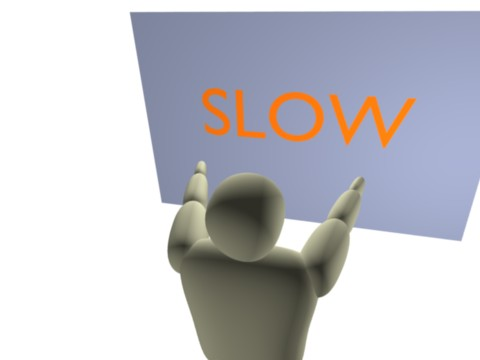
\includegraphics[width=5cm]{gfx/immi-fly-slow.jpg}
		\caption{control flight speed}
		\label{fig:fly-speed}
\end{figure}

\begin{figure}[!ht]
		\centering
		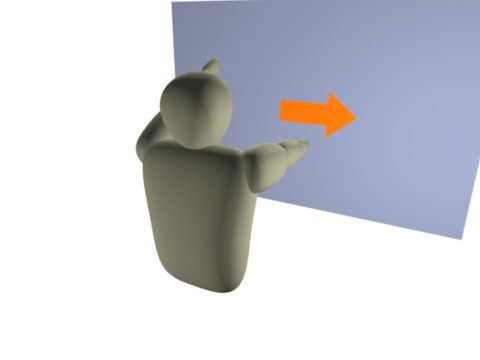
\includegraphics[width=5cm]{gfx/immi-fly-rotate.jpg}
		\qquad
		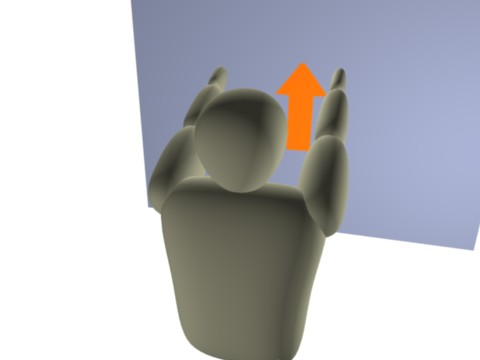
\includegraphics[width=5cm]{gfx/immi-fly-up.jpg}
		\caption{rotate flight orientation and increasing flight altitude}
		\label{fig:fly-rot-up}
\end{figure}

%
%\TODO{IMMI PAPER}
